%%%%%%%%%%%%%%%%%%%%%%%%%%%%%%%%%%%%%%%%%
% NIWeek 2014 Poster by T. Reveyrand
% www.microwave.fr
% http://www.microwave.fr/LaTeX.html
% ---------------------------------------
% 
% Original template created by:
% Brian Amberg (baposter@brian-amberg.de)
%
% This template has been downloaded from:
% http://www.LaTeXTemplates.com
%
% License:
% CC BY-NC-SA 3.0 (http://creativecommons.org/licenses/by-nc-sa/3.0/)
%
%%%%%%%%%%%%%%%%%%%%%%%%%%%%%%%%%%%%%%%%%

%----------------------------------------------------------------------------------------
%	PACKAGES AND OTHER DOCUMENT CONFIGURATIONS
%----------------------------------------------------------------------------------------

\documentclass[a0paper,portrait]{baposter}

\usepackage[font=small,labelfont=bf]{caption} % Required for specifying captions to tables and figures
\usepackage{booktabs} % Horizontal rules in tables
\usepackage{relsize} % Used for making text smaller in some places

\usepackage{amsmath,amsfonts,amssymb,amsthm, stmaryrd} % Math packages
\usepackage{eqparbox}

\usepackage{textcomp}


\graphicspath{{figures/}} % Directory in which figures are stored

 \definecolor{bordercol}{RGB}{40,40,40} % Border color of content boxes
 \definecolor{headercol1}{RGB}{186,215,230} % Background color for the header in the content boxes (left side)
 \definecolor{headercol2}{RGB}{120,120,120} % Background color for the header in the content boxes (right side)
 \definecolor{headerfontcol}{RGB}{0,0,0} % Text color for the header text in the content boxes
 %\definecolor{boxcolor}{RGB}{210,235,250} % Background color for the content in the content boxes
 \definecolor{boxcolor}{RGB}{255,255,255}
 
 \usepackage{algorithm}
\usepackage[noend]{algpseudocode} 

\usepackage[all,pdftex]{xy}
% For faster compilation. Entries must be wrapped in curly braces!
\CompileMatrices 
\xyoption{v2}
\xyoption{curve}
\xyoption{2cell}
\SelectTips{cm}{}  % Tips (of arrows) are in accordance with Computer Modern
\UseAllTwocells
%\SilentMatrices
\def\labelstyle{\textstyle}
\def\twocellstyle{\textstyle}

\newcommand{\bu}{\mathbf{u}}
\newcommand{\bv}{\mathbf{v}}

% define some signal names as abbreviations
\newcommand{\throttle}{\mathit{throttle}}
\newcommand{\brake}{\mathit{brake}}
\newcommand{\speed}{\mathit{speed}}
\newcommand{\rpm}{\mathit{rpm}}
\newcommand{\gear}{\mathit{gear}}
\newcommand{\AF}{\mathit{AF}}
\newcommand{\AFref}{\mathit{AF}_\text{ref}}

\newcommand{\DiaOp}[1]{\Diamond_{#1}}
\newcommand{\BoxOp}[1]{\square_{#1}}

\newcommand{\yes}{20*}
\newcommand{\no}{0*}

\newcommand{\Falsify}{\mathsf{Falsify}}
\newcommand{\STL}{\textbf{STL}}
\newcommand{\Rpos}{\R_{>0}}
\newcommand{\R}{{\mathbb{R}}}
\newcommand{\N}{{\mathbb{N}}}


\DeclareMathOperator*{\argmin}{arg\,min}

\newcommand{\sem}[1]{\llbracket #1 \rrbracket} 

\begin{document}

\background{ % Set the background to an image (background.pdf)
\begin{tikzpicture}[remember picture,overlay]
\draw (current page.north west)+(-2em,2em) node[anchor=north west]
{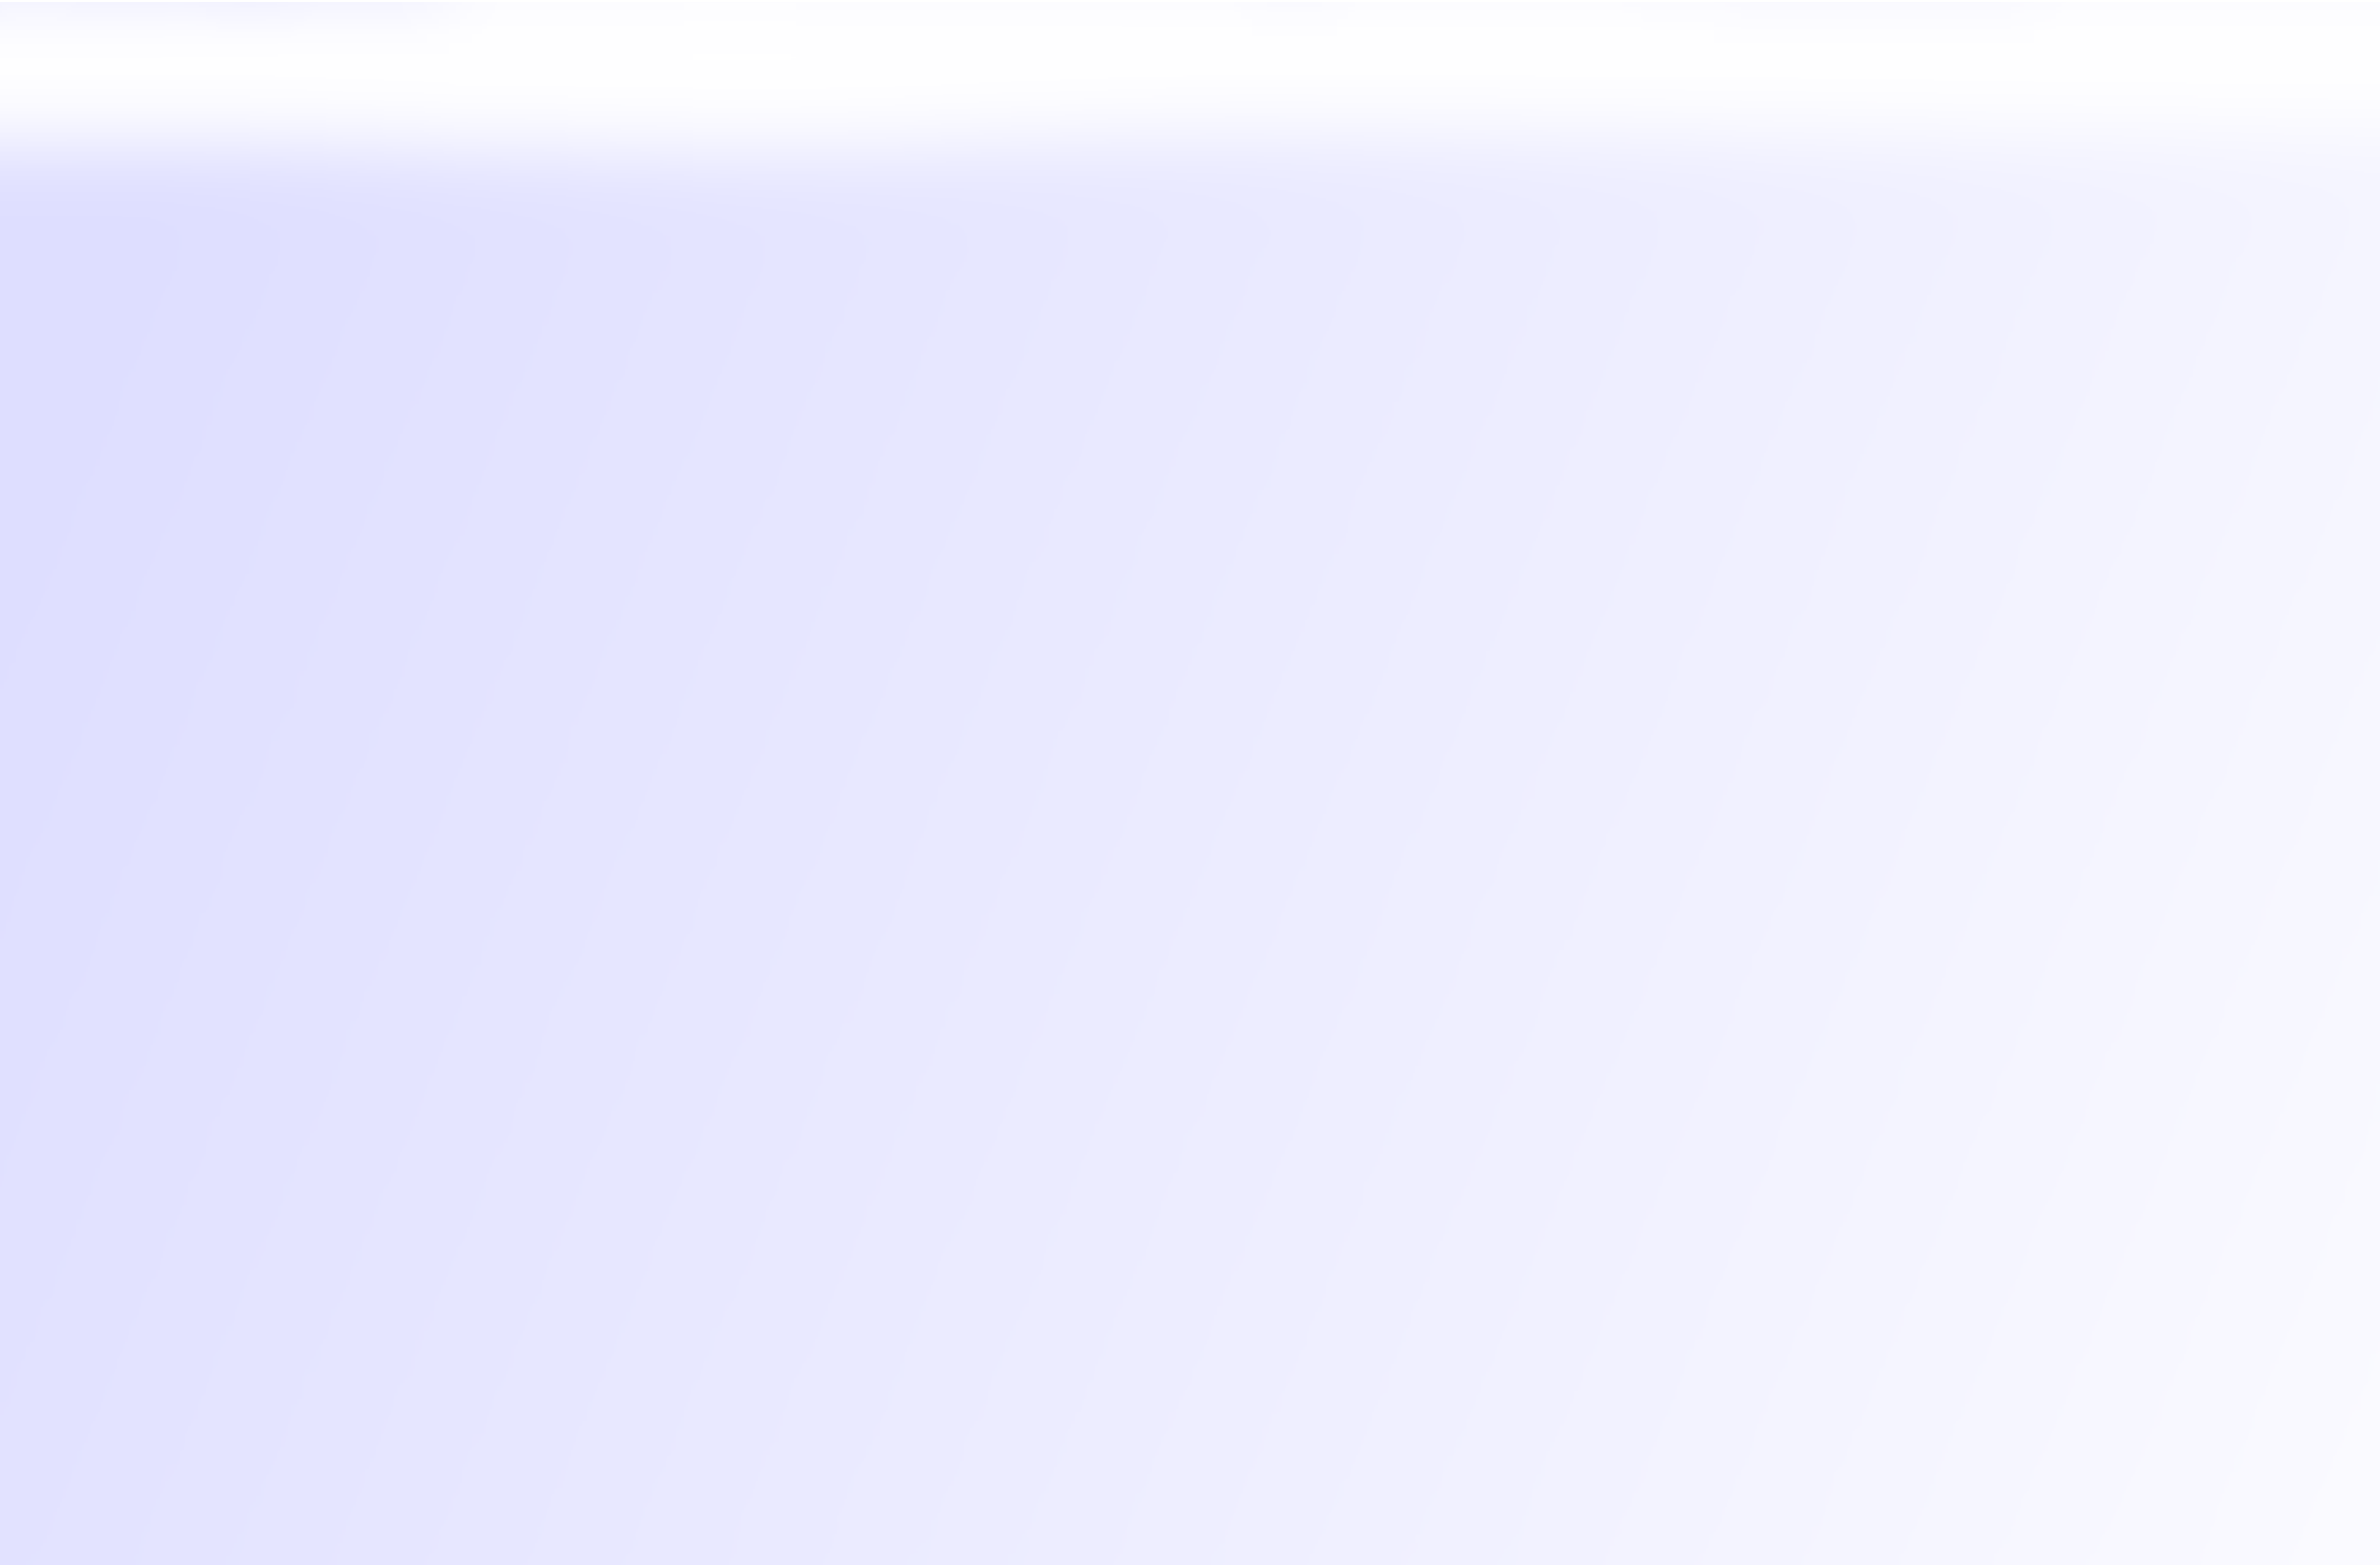
\includegraphics[height=1.1\textheight]{background}};
\end{tikzpicture}
}

\begin{poster}{
grid=false,
borderColor=bordercol, % Border color of content boxes
headerColorOne=headercol1, % Background color for the header in the content boxes (left side)
headerColorTwo=headercol2, % Background color for the header in the content boxes (right side)
headerFontColor=headerfontcol, % Text color for the header text in the content boxes
boxColorOne=boxcolor, % Background color for the content in the content boxes
headershape=roundedright, % Specify the rounded corner in the content box headers
headerfont=\Large\sf\bf, % Font modifiers for the text in the content box headers
textborder=rectangle,
background=user,
headerborder=open, % Change to closed for a line under the content box headers
boxshade=plain
}
{
\includegraphics[scale=0.2]{erato.png}}
%
%----------------------------------------------------------------------------------------
%	TITLE AND AUTHOR NAME
%----------------------------------------------------------------------------------------
%
{\huge    {Time-Staging Enhancement of Hybrid System Falsification} } % Poster title
{\vspace{0.3em} \smaller Gidon Ernst$^1$, Ichiro Hasuo$^1$, Sean Sedwards$^2$, Zhenya Zhang$^1$  \\  % Author names
  
\smaller $^1$\it {National Institute of Informatics, Tokyo, Japan} \\ $^2$\it{University of Waterloo, Waterloo, Canada} } % Author email addresses
%{
\includegraphics[scale=0.45]{NI.jpg}} % University/lab logo

%----------------------------------------------------------------------------------------
%	INTRODUCTION
%----------------------------------------------------------------------------------------
\headerbox{Problem}{name=introduction,column=0,row=0, span=3}{

\begin{itemize}



\item Falsification problem is defined as follows:
%In formal verification one aims to give a mathematical proof for a system's correctness. This is much harder for hybrid systems than for computer software/hardware, %. One reason is theoretical:
% where the presence of continuous dynamics makes many problems more complex or even undecidable (e.g.\ reachability in hybrid automata). 
% \begin{minipage}{0.65\textwidth}
%    \underline{\bfseries The falsification problem}
\vspace{-0.5em} 
    \begin{itemize}
    \item{\textbf{Given:}} 
      a \emph{model} $\mathcal{M}$ (that takes an input signal $\bu$
      and  yields  an output signal $\mathcal{M}(\bu)$), and
      a \emph{specification} $\varphi$ (a temporal formula) 
    \item{\textbf{Answer:}} 
      \emph{error input}, that is, an input signal $\bu$ such
      that the corresponding output $\mathcal{M}(\bu)$ violates $\varphi$ 
    \end{itemize}
 % \end{minipage}




\item Challenges:
\vspace{-1.1em} 

\begin{itemize}
	\vspace{-0.3em} 
\item Black/Grey box model, e.g., model in Simulink, etc.
\begin{minipage}{0.3\textwidth}
\centering
  \begin{math} 
   \xymatrix@1@+1.5em{
   {}
     \ar[r]^-{\bu}
   &
   {  \quad\xybox{ *+++[F]{\mathcal{M}} }}
     \ar[r]^-{\mathcal{M}(\bu)}_-{\not\models\varphi \; ?}
   &
   {}
   }
  \end{math}
 \end{minipage}
\vspace{-0.8em} 
\item Continuous (infinite) input space
\end{itemize}
\end{itemize}

}


%----------------------------------------------------------------------------------------
%	CALIBRATION
%----------------------------------------------------------------------------------------
\headerbox{Related work}{name=relwork, column=0, below=introduction}{
\begin{itemize}
\item Robust semantics of temporal formulas
\begin{itemize}
\item Traditional: Boolean satisfaction relation $\bv\models\varphi$
\item Now: quantity $\sem{\bv,\varphi}\in\R\cup\{\infty,-\infty\}$ $\sem{\mathbf{v}_2,\varphi} = -10$
\end{itemize}


\item Optimization-based falsification: 
\begin{itemize}
\item Objective function: $\sem{\bv,\varphi}$
\item Solvers: Nelder-Mead, CMA-ES, Simulated Annealing, etc. $\sem{\mathcal{M}(\bu^{(i+1)}),\varphi} > \sem{\mathcal{M}(\bu^{(i)}),\varphi}$    
\end{itemize}

\end{itemize}

}




\headerbox{Motivating example}{name=optsolver, column=0, below=relwork}{
\vspace{0.6em}

\quad  $\bullet \quad\Box~(\speed < 120)$

\vspace{1em}

  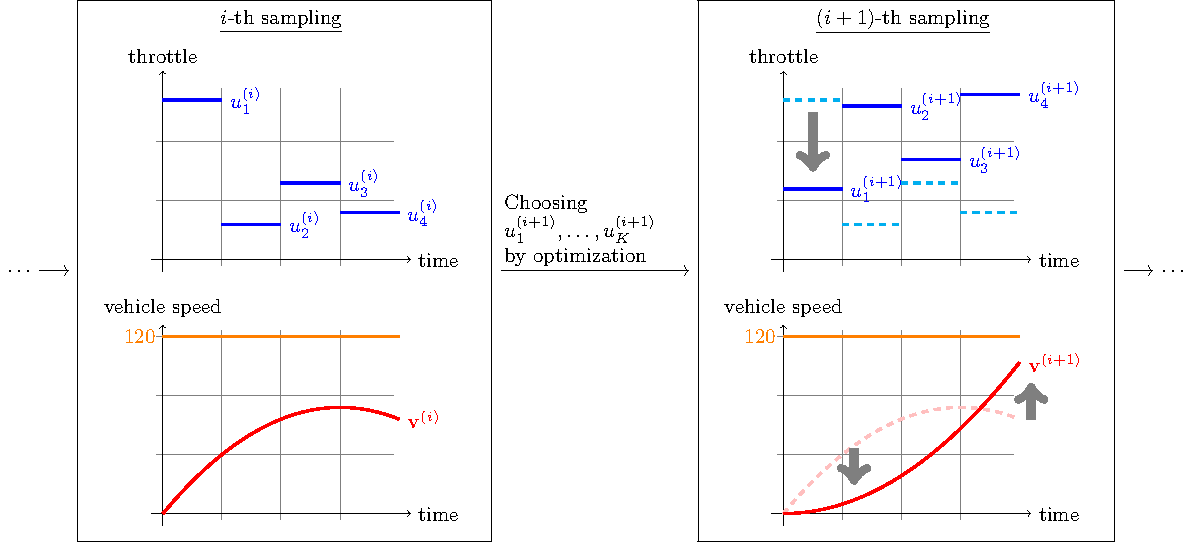
\includegraphics[scale=.3]{figures/figUnstagedFalsification.pdf}\centering
  \begin{itemize}
\item In the $i$-th sampling one tries an input signal $\bu^{(i)}$. The corresponding output signal $\bv^{(i)}=\mathcal{M}(\bu^{(i)})$ is shown below it.
\vspace{-0.3em}
\item Optimization algorithm decides a new input signal 
$\bu^{(i+1)}=(u_{1}^{(i+1)},\dotsc,u_{K}^{(i+1)})$. %It is in the choice
and $\bu^{(i+1)}$ makes the robustness smaller (i.e.\ the peak vehicle speed higher). 
\end{itemize}

  
}

\headerbox{Time-staged strategy}{name=overview, column=0, below=optsolver}{
\vspace*{0.6em}
\centering
 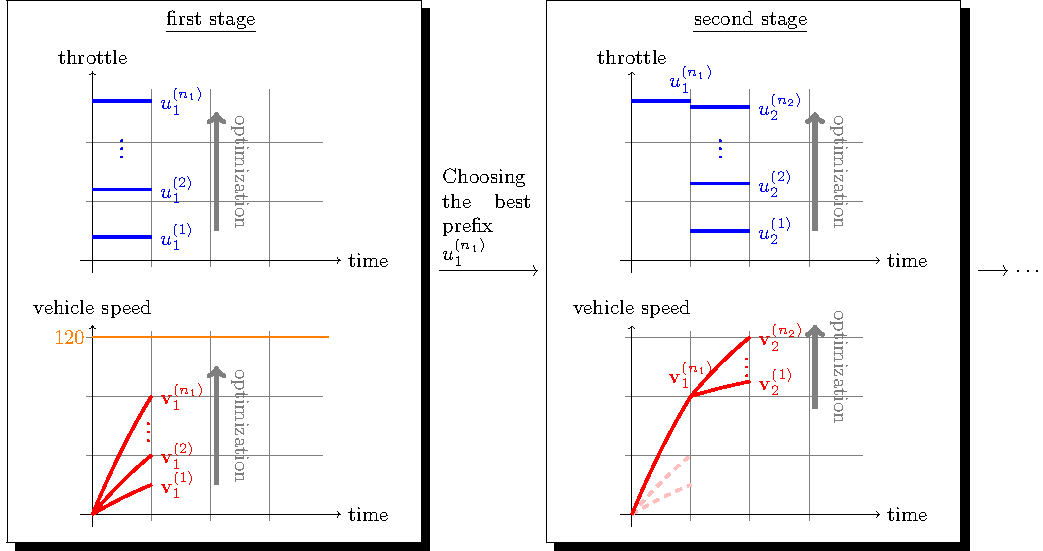
\includegraphics[scale=.4]{figures/figStagedFalsification.pdf}
 
 \begin{itemize}
\item In the first stage (left), we run a falsification algorithm and try to find an initial input segment that achieves low robustness (i.e.\ high peak speed). \vspace{-0.3em}
\item This process will gradually improve candidates for the initial input segment, in the way the  arrows $\uparrow$ on the left in the figure designate. 
\end{itemize}

 

 
}


%----------------------------------------------------------------------------------------
%	OTHER INSTRUMENTATION
%----------------------------------------------------------------------------------------
\headerbox{Time-staged falsification algorithm}{name=algorithm,span=2,column=1,row=1, below=introduction}{ % To reduce this block to 1 column width, remove 'span=2'


%\begin{algorithm}[t]


\begin{algorithmic}[1]
\Require a falsification solver $\Falsify$, a system model $\mathcal{M}$, an $\STL$ formula $\varphi$,  $T\in\Rpos$ and $K\in\N$
\State $\bu\gets ()$  
   \Comment{the input prefix obtained so far. We start with the empty signal $()$}
\For {$j \in \{1,\dotsc,K\}$}
\State $\bu'\gets \Falsify(\mathcal{M}_{\bu},\partial_{\mathcal{M}(\bu)}\rho_{\varphi}, \frac{T}{K})$
   \Comment{synthesizing the $j$-th input segment}
\label{line:jthStage}
\State $\bu\gets \bu\cdot \bu'$ 
   \Comment{concatenate $\bu'$, after which the length of $\bu$ is $\frac{jT}{K}$}
\EndFor
\State \Return $\bu$
 \Comment{a time-staged falsification trial is successful if $\sem{\mathcal{M}(\bu),\varphi} < 0$}
% \While {$\lnot\mathsf{InitialSamplingDone}(T,\mathcal{U})$} 
%  \State $\bu\gets\mathsf{InitialSampling}(T)$
%        \Comment{ $\bu\colon [0,T]\to \R^{M}$ is sampled following some recipe}         
%  \State $\mathcal{U}\gets \mathsf{cons}(\mathcal{U},\bu)$
% \EndWhile
% \While {$\lnot\mathsf{OptimizationSamplingDone}(\mathcal{M},\varphi,T,\mathcal{U})$}
%   \State $\bu\gets\mathsf{OptimizationSampling}(\mathcal{M},\varphi,T,\mathcal{U})$
%     \State 
%      \Comment{\parbox[t]{.92\linewidth}{
%            $\bu$ is sampled, so that $\sem{\mathcal{M}(\bu),\varphi}$ gets small,
%            based on  previous samples in $\mathcal{U}$}}
%  \State $\mathcal{U}\gets \mathsf{cons}(\mathcal{U},\bu)$
% \EndWhile
% \State $\bu\gets\argmin_{\bu\in\mathcal{U}}\sem{\mathcal{M}(\bu),\varphi}$
% \State \Return $\bu$
%  \Comment{a trial is successful if $\sem{\mathcal{M}(\bu),\varphi} < 0$}
\end{algorithmic}
%\end{algorithm}

}


%----------------------------------------------------------------------------------------
%	MIXER vs. SAMPLERS
%----------------------------------------------------------------------------------------
\headerbox{Benchmark 1: Automatic transmission}{name=autotrans, span=2, column=1, row=1, below=algorithm}{

%\begin{small}\centering

\scalebox{0.88}{
\begin{tabular}{|r||rr|rr||rr|rr||rr|rr||}
%\hline
 %      model
    %   & \multicolumn{12}{c||}{Automatic Transmission}
       %& \multicolumn{4}{c|}{Abst.\ Fuel Ctrl.}
     %  \\
\hline
   %    spec.\
       & \multicolumn{2}{c|}{S1}
       & \multicolumn{2}{c||}{S2}
       & \multicolumn{2}{c|}{S3 easy}
       & \multicolumn{2}{c||}{S3 hard}
       & \multicolumn{2}{c|}{S4 easy}
      % & \multicolumn{2}{c|}{S4 mid}
       & \multicolumn{2}{c||}{S4 hard}
      % & \multicolumn{2}{c|}{S init}
     %  & \multicolumn{2}{c|}{S stable}
       \\
\hline
Algorithm
  & time & \#/20
  & time & \#/20
  & time & \#/20
  & time & \#/20
%  & time & \#/20
  & time & \#/20
%  & time & \#/20
%  & time & \#/20
  & time & \#/20 \\
\hline
CMA-ES & 27s & \textbf{20}   &  \textbf{5s} & \textbf{20}
       & 39s & 14 & 57s &  0
       & 32s & 16  & 59s &  0
       %& 49s &  0 & 82s &  1
       \\
   +TS & 52s & 15   & 15s & 16
       & \textbf{9s} & 19 & 23s & \textbf{11}
       & 15s & 14  & 24s &  3
     %  & 30s &0    &  42s & 1
       \\
 +A-TS & 41s & 18   & 15s & 17
       & \textbf{9s} & 16 & 21s & \textbf{10}
       & 26s & 14  & \textbf{20s} &  \textbf{5}
    %   & 26s& 0    & 41s & 0
       \\
\hline
    SA & 50s & 5    & 43s &  7
       & 37s &  9 & 55s &  0
       & 35s &  6  & 47s &  \textbf{5}
      % & 51s & 0   & 76s & 2
       \\
   +TS & 37s & \textbf{20}   & 33s & \textbf{16}
       & \textbf{11s} & \textbf{19} & 33s &  \textbf{8}
       & 21s & 14  & 51s &  0
    %   & 47s & \textbf{1}   & 54s & \textbf{7}
       \\
 +A-TS & 34s & \textbf{20}   & 18s & \textbf{17}
       &  \textbf{9s} & \textbf{18} & 26s &  \textbf{4}
       & \textbf{16s} & \textbf{18}  & 30s &  2
    %   & 34s & 0   & 42s & \textbf{5}
       \\
\hline      
   GNM &\textbf{6s} & \textbf{\yes} & 61s & \no
       & 56s & \no & 55s & \no
       & 43s & \no &  53s & \no
     %  & 50s & \no & 86s & \no
       \\
   +TS & 42s & \yes & 15s & \textbf{\yes}
       & \textbf{13s} & \textbf{\yes} & 25s & \textbf{\yes}
       & \textbf{11s} & \textbf{\yes} & 52s & \no
      % & 30s &\textbf{\yes}  & \textbf{20s} &\textbf{\yes}
       \\
 +A-TS & 20s & \yes & 16s & \textbf{\yes}
       & \textbf{10s} & \textbf{\yes} & 26s & \textbf{\yes}
       & 13s & \yes  & 43s & \no
    %   & 37s & \no & \textbf{19s} & \textbf{\yes}
       \\
\hline
\end{tabular}
}

\textbf{S1} $\Box_{[0,30]}~(\speed < 120)$

\textbf{S2} $\Box_{[0,30]}~(\gear = 3 \to \speed \ge 30)$

\textbf{S3} $\Diamond_{[10,30]}~(\speed \le v_\text{min} \lor \speed \ge v_\text{max})$, easy: $v_\text{min}: 50$, $v_\text{max}: 60$;
hard:          $v_\text{min}: 53$, $v_\text{max}: 57$.


\textbf{S4} $\Box_{[0,10]}(v_\text{min} < \speed) \lor \Diamond_{[0,30]}(\rpm > \omega_\text{max})$ \begin{small}easy: $v_\text{min}: 80, \omega_\text{max}: 4500$;
hard:          $v_\text{min}: 50, \omega_\text{max}: 2520$. \end{small}


%\end{small}
}


%----------------------------------------------------------------------------------------
%	MEASUREMENT SETUP
%----------------------------------------------------------------------------------------
\headerbox{Benchmark 2: Abstract fuel control}{name=afc,span=2,column=1,below=autotrans}{ 

\begin{small}
\begin{tabular}{|r||rr|rr|rlr|}
\hline
       & \multicolumn{2}{c|}{$\neg(\DiaOp{[0,6]}{\BoxOp{[0,3]}{(\AF - \AFref > 0.07 * 14.7))}}$}
       & \multicolumn{2}{c|}{$\neg(\DiaOp{[6,26]}{\BoxOp{[0,4]}{(\AF - \AFref > 0.01 * 14.7))}}$}
	\\
\hline
Algorithm
  & time& \#/20
  & time& \#/20 \\
\hline
     CMA-ES & 49s &0   &   82s & 1 \\
  +TS & 30s &0    &  42s & 1 \\
+A TS& 26s& 0    & 41s & 0 \\
\hline                    
     SA     & 51s & 0   & 76s & 2  \\
  +TS  & 47s & 1   & 54s & 7 \\
+A TS& 34s & 0   & 42s & 5 \\
\hline      
     GNM    & 50s & \no & 86s & \no\\
  +TS & 30s &\yes  & 20s &\yes \\
+A TS& 37s & \no & 19s & \yes \\
\hline
\end{tabular}
\end{small}
}



%----------------------------------------------------------------------------------------
%	CONCLUSION
%----------------------------------------------------------------------------------------
\headerbox{Conclusion \& Future work }{name=conclusion,column=1,below=afc,span=2}{
We have introduced and evaluated the idea of time staging to enhance
falsification for hybrid systems. The proposed method emphasizes exploitation
over exploration as part of stochastic optimization.
As there is no single algorithm that fits every problem
(as a consequence of having no free lunch),
having a variety of methods at disposal permits the user of a system
to choose the one suitable for the problem at hand.
We have shown that the proposed approach is a good fit for problems that suitable exhibit
time-causal structures, where it significantly outperforms non-staged algorithms.

\vspace{0.85em}
Three directions for future work:
\begin{itemize}
\vspace{-0.3em}
\item Instead of just picking the best trajectory for each stage,
it might be beneficial to retain a few, potentially diverse ones.
\vspace{-0.3em}
\item Discover time stages adaptively.
\vspace{-0.3em}
\item Explore variations of robust semantics
to mitigate discrete propositions.
\end{itemize}


}


%----------------------------------------------------------------------------------------
%	REFERENCES
%----------------------------------------------------------------------------------------

%\headerbox{References}{name=references,column=2,below=application}{

%\smaller % Reduce the font size in this block
%\renewcommand{\section}[2]{\vskip 0.05em} % Get rid of the default "References" section title
%\nocite{*} % Insert publications even if they are not cited in the poster

%\bibliographystyle{unsrt}
%\bibliographystyle{IEEEtran}
%\bibliography{biblio} % Use biblio.bib as the bibliography file
%}


%----------------------------------------------------------------------------------------
%	ACKNOWLEDGEMENTS
%----------------------------------------------------------------------------------------

\headerbox{Acknowledgements}{name=acknowledgements,column=0,below=conclusion , above=bottom,span=3}{

This work is supported by ERATO HASUO Metamathematics for Systems Design Project
(No. JPMJER1603), Japan Science and Technology Agency.
} 


\end{poster}

\end{document}